% 2010 年北京卷理科第 17 题：正方形 ABCD 与四边形 ACEF 所在平面互相垂直。
% 来源 PDF：普通高考/2010/2010北京理.pdf，SHA-256 6b5819672aaf59aecfce92e08c2d045a80575803527d61813497dd669a8d5529。
% 原页：第 2 页（A3 三栏）第 1 栏上部，书页码 576。
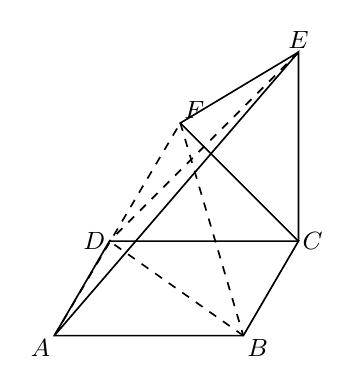
\begin{tikzpicture}[semithick, every node/.style={inner sep=1.2pt, font=\small}]
  \coordinate (A) at (0,0);
  \coordinate (B) at (2.4,0);
  \coordinate (C) at (3.1,1.2);
  \coordinate (D) at (0.7,1.2);
  \coordinate (E) at (3.1,3.6);
  \coordinate (F) at (1.6,2.7);
  % 底面
  \draw (A) -- (B) -- (C) -- (D) -- cycle;
  % 四边形 ACEF
  \draw (A) -- (E) -- (C);
  \draw[dashed] (A) -- (F);
  \draw (E) -- (F) -- (C);
  \draw[dashed] (F) -- (B);
  \draw[dashed] (E) -- (D);
  \draw[dashed] (B) -- (D);
  % 标注
  \node[below left] at (A) {$A$};
  \node[below right] at (B) {$B$};
  \node[right] at (C) {$C$};
  \node[left] at (D) {$D$};
  \node[above] at (E) {$E$};
  \node[above right] at (F) {$F$};
\end{tikzpicture}
